\documentclass[11pt,a4paper,twoside]{article}
\usepackage[includeheadfoot, left=3cm, right=2cm, top=2.5cm, bottom=2.5cm, headheight=19.3pt]{geometry}

\usepackage[polish]{babel}
\usepackage[T1]{fontenc}
\usepackage[utf8]{inputenc}
\usepackage[scaled]{helvet}
\renewcommand\familydefault{\sfdefault} 

\let\lll=\relax
\usepackage{amsmath}
\usepackage{amsfonts}
\usepackage{amssymb}
\usepackage{bm}

\usepackage{url}
\usepackage{pdfpages}
\usepackage[bookmarks, pagebackref]{hyperref}
\usepackage[none]{hyphenat}
\usepackage{graphicx}
\usepackage{color}
\usepackage{array}
\usepackage{etoolbox, fancyhdr, xcolor}
\usepackage[hang, flushmargin]{footmisc}
\usepackage{setspace}
\usepackage{ragged2e}
\usepackage{MnSymbol}
\usepackage[nottoc]{tocbibind}
\usepackage{titlesec}
\urlstyle{rm}
\usepackage[ampersand]{easylist}
\usepackage{enumitem}
\setlist[itemize]{noitemsep, topsep=0pt, leftmargin=*, itemindent=-1cm}
\usepackage{epsfig}
\usepackage{float}
\usepackage[font={up, footnotesize}, labelfont=bf, singlelinecheck=off, format=hang]{caption}
\usepackage{caption}
\usepackage{subcaption}
\usepackage{listings}
\lstset{language=C++, rulecolor=\color{sapphire}, framerule=1.5pt} % you can change language of your code
\usepackage{colortbl}
\usepackage{tabu}
\usepackage{makecell}
\usepackage{boldline}
\setlength{\arrayrulewidth}{1pt}
\captionsetup[table]{name=Tabela}

\usepackage{lipsum} % for testing purposes

\definecolor{sapphire}{RGB}{120,150,207}
\definecolor{grafit}{RGB}{60,60,60}

% pdf output setup
\hypersetup{
	unicode,
	pdftoolbar,
	pdfmenubar,
	pdffitwindow,
	pdfstartview = {FitH},
	pdftitle = {Praca Inżynierska}, 
	pdfauthor = {Ahata Valiukevich},
	pdfnewwindow,
	colorlinks,
	linktoc = page,
	% use color sapphire or grafit
	linkcolor = sapphire,
	citecolor = sapphire,
	filecolor = sapphire,
	urlcolor = black
}


\newcommand{\itemi}[1][sapphire]{\item[\color{#1} $\filledsquare$]}
\newcommand{\itemii}[1][sapphire]{\item[\color{#1} $\square$]}
\newcommand{\itemiii}[1][sapphire]{\item[\color{#1} $\bullet$]}

\ListProperties(Hide=100, Progressive=1cm, Style=\color{sapphire}, Style**=\color{black}, Style*=$\square$ ,Style2*=$\bullet$)


\newcommand{\headrulecolor}[1]{\patchcmd{\headrule}{\hrule}{\color{#1}\hrule}{}{}}
\newcommand{\footrulecolor}[1]{\patchcmd{\footrule}{\hrule}{\color{#1}\hrule}{}{}}


\newcommand{\infostyle}[1]
{
	\fancyhf{}
	\fancyhead[LO]{\Large{\textbf{#1}}}

	\renewcommand{\headrulewidth}{1.5pt}
	\headrulecolor{sapphire}
	\justify
	\pagestyle{fancy}
}


\newcommand{\thesisstyle}
{
	\fancyhf{}
	\fancyhead[RO,LE]{\Large{\textbf{\rightmark}}}
	\fancyfoot[LE,RO]{\thepage}

	\renewcommand{\headrulewidth}{1.5pt}
	\renewcommand{\footrulewidth}{1.5pt}
	\headrulecolor{sapphire}
	\footrulecolor{sapphire}
	\justify
	\pagestyle{fancy}
}


\newcommand{\fancyfootnotetext}[2]
{
	\fancypagestyle{footnotes}
	{
    	\fancyfoot[LO,RE]{\parbox{15cm}{\footnotemark[#1]\footnotesize #2}}
	}
	\thispagestyle{footnotes}
}


\newcommand{\fancyfootnotetexts}[4]
{
	\fancypagestyle{footnotes}
	{
    	\fancyfoot[LO,RE]{\parbox{15cm}{\footnotemark[#1]\footnotesize #2 \\ \footnotemark[#3]\footnotesize #4}}
	}
	\thispagestyle{footnotes}
}


\newcommand{\fancyfootnotetextss}[6]
{
	\fancypagestyle{footnotes}
	{
    	\fancyfoot[LO,RE]{\parbox{15cm}{\footnotemark[#1]\footnotesize #2 \\ \footnotemark[#3]\footnotesize #4 \\ \footnotemark[#5]\footnotesize #6 \\}}
	}
	\thispagestyle{footnotes}
}


\titlespacing\section{0pt}{15pt}{10pt} 
\titlespacing\subsection{0pt}{15pt}{10pt} 
\titlespacing\subsubsection{0pt}{15pt}{10pt} 

\setstretch{1.15}
\setlength{\parindent}{0.5cm} 
\setlength{\parskip}{0cm} 

\frenchspacing
\sloppy

\author{} 
\title{} 
\date{}
\graphicspath{{images/}}
\begin{document}

\includepdf[pages={-}]{preamble/begining.pdf}
\tableofcontents
\thispagestyle{empty}
\thesisstyle
\newpage 

\section[Wstęp]{Wstęp}
W przeciągu ostatnich kilku lat nauka zrobiła duży postęp w kierunku rozwoju fizyki dużych energii. Osiągnięcie to składa się z wyników dużej liczby badań oraz eksperymentów prowadzonych w różnych naukowo-badawczych instytucjach. Równolegle z naukami fizycznymi rozwiajała się również branża informatyczna, a w szczególności grafika komputerowa. Obecnie jest obserwowany coraz silniejszy trend związany z rozwojem technik stereoskopowych. Przy połączeniu badań fizycznych i grafiki komputerowej powstaje możliwość dogłębnego przestudiowania zjawisk zachodzących podczas rożnych eksperymentów.

\subsection{Cele i zakres pracy}
Pierwszym celem niniejszej pracy dyplomowej jest stereoskopwa wizualizacja detektora oraz zdarzeń ciężkich ionów w eksperymencie ALICE. Kolejnym istotnym celem pracy jest połączenie wyżej wymienionych wizualizacji do jednego spójnego obrazu. \\
Dla realizacji celi podstawowych niezbędne jest zapoznanie się z technologią stereoskopii i aktualnie dostępnymi rozwiązaniami, przestudiowanie podstaw działania eksperymentu ALICE oraz środowiska informatycznego w CERN.\\
Celem pośrednim danej pracy jest zapoznanie się z możliwościami biblioteki OpenGL, a także innymi uwarunkowaniami ważymi w aspekcie projektowanej aplikacji.

\newpage
\section[Część analityczna]{Część analityczna}

\subsection{Stereoskopia}
Stereoskopia - to technika służącą do tworzenia iluzji głębi obrazu, nie zapewnia ona prawdziwie trójwymiarowych widoków, ale zapewnia efekt trójwymiarowości. Sceny wydają się mieć głębię, ponieważ każdemu oku obserwatora jest prezentowany inny widok. \\
Istnieje kilka różnych technik osiągnięcia efektu stereoskopowego. Dla każdego rodzaju przeglądania niezbędny jest materiał stereoskopowy dostosowany do konkretnego celu. W dalszej części niniejszej pracy są przedstawione krótkie opisy kilku technik cieszących się dużą rozpoznawalnością. Niektóre z nich są odpowiednie tylko dla jednego widza, podczas gdy istnieją różne typy okularów 3D sprawdzające się dla większej grupy odbiorców.
\subsubsection{Historia} 
Historia stereoskopii liczy już ponad 180 lat. Za odkrywcę tej techniki uważa się Charlesa Wheatstone'a, który jako pierwszy zaobserwował zjawisko widzenia stereoskopowego, opisał go w artykule \cite{wheatstone} oraz skonstruował urządzenie potwierdzające słuszność jego teorii \cite{stereoscopehistory}.\\
Wheatstone wyjaśnia, że jeśli obiekt znajduje się w małej odległości od oczu, to każde oko widzi przedmiot pod nieco innym kątem, z innej perspektywy. Zaś dla obiektów na dużej odległości nie ma to znaczenia. Wykorzystując te obserwacje, autor skonstruował urządzenie, które umożliwiło przedstawienie delikatnie różniących się obrazów prawemu i lewemu oku z osobna z powstającą w efekcie iluzją trójwymiarowości obrazu.

\subsubsection{Stereogramy typu side by side}
Najprostszą metodą doświadczenia widzenia stereoskopowego jest umieszczenie dwuch oddzielnych obrazów obok siebie. Perspektywa jednego z obrazów reprezentuje lewe oko, odpowiednio druga perspektywa jest dla oka prawego. Obrazy te można zazwyczaj oglądać bez użycia dodatkowych narzędzi. Jedyna różnica polega na sposobie ich oglądania. Jeśli obraz dla lewego oka znajduje się po lewej stronie, to stosuje się technikę patrzenia równolegległego, w innym przypadku obrazy mają być oglądane z użyciem techniki skrośnej. Zastosowanie niewłaściwej metody spowoduje odwrócenie efektu stereoskopowego. Może to ujawnić się w postaci zniekształconych odległości pomiędzy obiektami na obrazie lub oddalenia się dwóch obrazów. \\
Warto zauważyć, że oglądanie stereogramów tworzy duże obciążenie dla oczu. W celu zmniejszenia negatywnych skutków używa się stereoskopu bądź specjalnego ekranu 3D z okularami. To w znacznej mierze redukuje przemęczenie oczu i pozwala przez dłuższy czas przyglądać się efektom widzenia stereoskopowego.
\footnote{http://blogs.hebali.com/itp/?p=378}
\begin{figure}[H]
		\centering
 		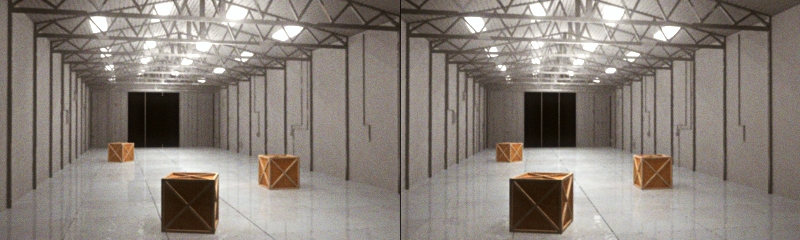
\includegraphics[width=10cm]{sbs.jpg}
 		\captionsetup{font={up, footnotesize}}
    	\caption{Stereogram.}
 		\label{rys1}
\end{figure}

\subsubsection{Stereogramy typu single-image} 
Stereogramy typu single-image, inaczej nazywane autostereogramy, to zbiór punktów, które wydają się tworzyć trójwymiarową scenę, gdy są skrośnie oglądane z bliska. Do osiągnięcia efektu stereoskopowego za pośrednictwem autostereogramów nie są potrzebne żadne urządzenia, aczkolwiek okulary pryzmatyczne ułatwiają przegladanie poprzeczne, a także nad- i podgląd.\\
Pzy użyciu poprawnej techniki oglądania specjalnie stworzonego obrazu powstaje wrażenie trójwymiarowości. Czasem obrazy mogą wyglądać jak zniekształcone lub losowo umieszczone kolorowe plamy. "Bałagan"\ tego rodzaju w rzeczywistości nie jest przypadkowy, ponieważ poprzez użycie powtarzalnego wzoru są ukrywane obiekty trójwymiarowe \cite{stereoscopythesis}.
\begin{figure}[H]
		\centering
 		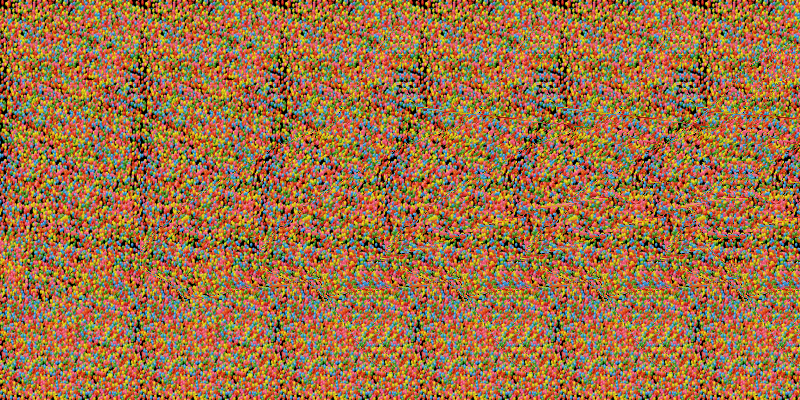
\includegraphics[width=10cm]{autostereogram.png}
 		\captionsetup{font={up, footnotesize}}
    	\caption{Autostereogram.}
 		\label{rys2}
\end{figure}

\subsubsection{Stereoskopia pasywna} 
Do tworzenia iluzji obrazów trójwymiarowych są wykorzystywane specjalnie spolaryzowane okulary, ograniczające światło docierające do każdego oka. W celu przedstawienia widoku stereoskopowego dwa obrazy są wyświetlane na tym samym ekranie z użyciem różnych filtrów polaryzacji. 
Istenieją 2 rodzaje filtrów: liniowe oraz kołowe.\\
W przypadku liniowej polaryzacji pole elektryczne światła jest skierowane pionowo bądź poziomo. Odbiorca zakłada odpowiednio dopasowane okulary, w których każda soczewka przepuszcza światło o innym kierunku polaryzacji. W ten sposób oczy obserwują różniące się obrazy. Minimalne pochylenie okularów może spowodować niezgodność polaryzacji światła a soczewek. Nieporządany efekt można wyeliminować korzystając z filtrów kołowych prawo- lub lewoskrętnych. Ruch ten pozostaje niezmienny, nawet jeśli okulary są dowolnie pochylone.\\
Niewątpliwą zaletą stereoskopii spolaryzowanej jest to, że wiele osób może oglądać obrazy stereoskopowe w tym samym czasie \cite{russianpage}. Wadą tego rozwiązania jest koszt specjalnego ekranu do wyświetlania obrazów. Taki ekran musi posiadać srebrną warstwę, dzięki czemu nie zniekształca się polaryzacja obrazów przy jednoczesnym wyświetlaniu.
\begin{figure}[H]
		\centering
 		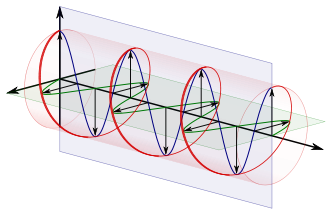
\includegraphics[width=8cm]{circular.png}
 		\captionsetup{font={up, footnotesize}}
    	\caption{Polaryzacja kołowa prawoskrętna.}
 		\label{rys3}
\end{figure}

\subsubsection{Stereoskopia aktywna} 
Możliwość oglądania obrazów stereoskopowych pojawia się dzięki ciekłokrystalicznym okularom migawkowym. Szkło, które tworzy soczewki okularów, zawiera ciekłe kryształy oraz filtr polaryzacyjny. Stosując napięcie można zmienić kolor soczewki na czarny, co bezpośrednio wiąże się z blokowaniem widoku dla jednego oka. Dzięki przykrywaniu widoku z dużą częstotliwością, każdemu oku są przedstawiane obrazy z różną perspektywą. Częstotliwość migotania okularów jest zsynchronizowana z aktualnym źródłem wyświetlania, żeby stale dostarczać prawidłowej perspektywy dla oczu. Jeśli prędkość aktualizacji soczewek w okularach nie jest wystarczająco wysoka, to może nastąpić zauważalne zniekształcenie obrazu końcowego. Przykładem takiego zniekształcenia może posłużyć część obrazu ze złą perspektywą, przeznaczona innemu oku. 

\subsubsection{Wizualizacja wielopasmowa}
Nowa technika wyświetlania obrazów stereoskopowych, znana też pod tytułem INFITEC - Interference filter technique. Opiera ona się na tym, że widmo światła widzialnego można podzielić na fale o różnej długości używając do tego filtrów optycznych \cite{infitec}.
 Światło widzialne jest podzielone na 6 części, po 2 na każdy z podstawowych kolorów: czerwony, zielony oraz niebieski. Poszczególne części przeznaczone są dla jednego oka, w ten sposób lekko różniące się barwy docierają do każdego oka z osobna. Wykorzystując fakt niewystarczającej wrażliwości mózgu do zauważenia tak niedużej różnicy, technika wizualizacji welopasmowej stwarza obrazy pełnokolorowe.  

\subsubsection{Techniki anaglifowe}
Do generowania stereogramu anaglifowego potrzebne są 2 obrazy z delikatnie różniącą się perspektywą dla każdego oka. Każdy obraz jest wykonany w podstawowych kolorach. Najbardziej popularną kombinacją jest obraz w kolorze czerwonym dla lewego oka i obraz wykonany w przy połączeniu zielonego i niebieskiego (otrzymany kolor nazywa się cyan) odpowiednio dla prawego oka. Obrazy umieszcza się jeden nad drugim. Efekt stereoskopowego widoku jest osiągany przy użyciu okularów z poprawnymi kolorowymi filtrami (podobnie jak obrazy: czerwony dla lewego oka, cyan dla prawego). Niestety przy użyciu tej techniki nigdy nie zostanie stworzony pełnokolorowy obraz, gdyż są ograniczone barwy widziane przez każde oko.\footnote{Wattie,John.Anaglyphs for computer stereoscopy.} \\
Istenieją tak że filtry o innych kolorach, zachowując główną zasadę anaglifów: przedstawienie innych obrazów każdemu oku poprzez ograniczenie pewnych barw. \\

\begin{figure}[H]
		\centering
 		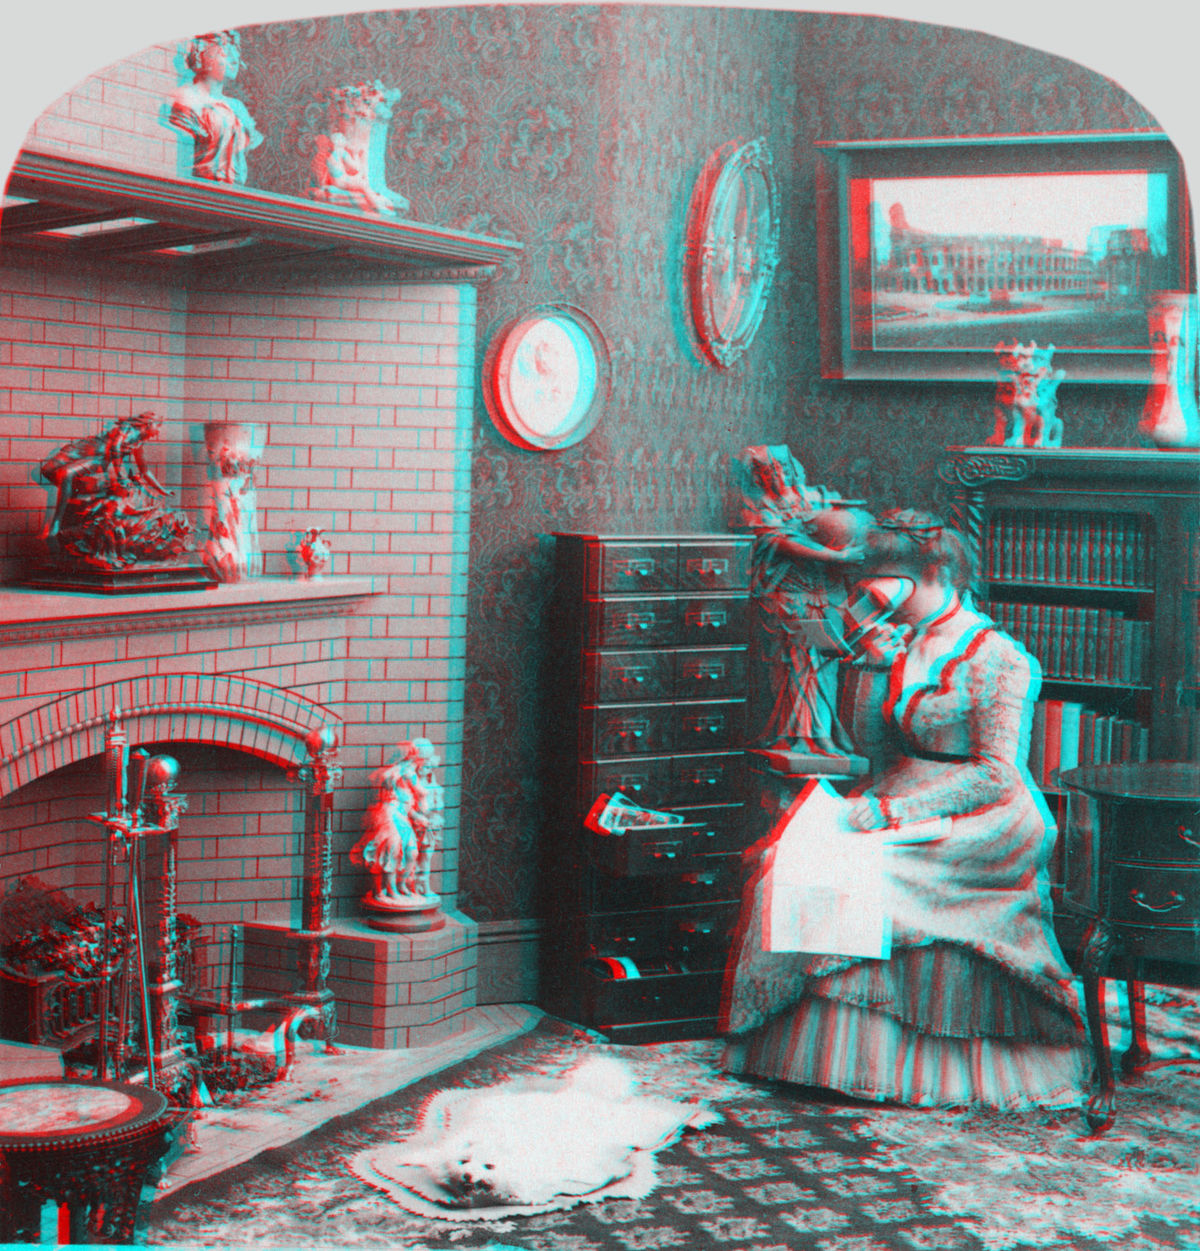
\includegraphics[width=6.5cm]{anaglif.jpg}
 		\captionsetup{font={up, footnotesize}}
    	\caption{Anaglif.}
 		\label{rys4}
\end{figure}

\newpage
\subsection{Formaty plików 3D}
W celu ponownego wykorzystania skonstruowanych modeli 3D i przesłania ich na różne platformy, tworzone są pliki graficzne. Jednak powstało wiele różnych formatów plików dla różnych aplikacji. Obecnie w grafice komputerowej istnieje ponad 70 odmiennych formatów%\footnote{https://en.wikipedia.org/wiki/List_of_file_formats#3D_graphics} 
. Są one wykorzystywane w różnych dziedzinach zaczynając od druku 3D, gier komputerowych, aż po medycynę i nauki przyrodnicze. \\
Podstawowym celem formatu pliku 3D jest przechowywanie informacji o modelu w postaci tekstu lub danych binarnych. W szczególności musi on zawierać dane o geometrii modelu, jego wyglądzie, scenie oraz animacjach. Geometria modelu opisuje jego dokładny kształt, do wyglądu zalicza się kolory, tekstury, typy wykorzystanych materiałów. Dane o scenie opisują między innymi położenie światła, kamery i obiektów pereferyjnych. \\
U podstaw każdego opragramowania graficznego znajduje się biblioteka niskiego poziomu, taka jak OpenGL czy Direct3D. Biblioteki niskiego poziomu faktycznie rysują modele 3D na ekranie. Modele mogą być również przechowywane i przesyłane jako pliki graficzne. Narzędzia autorskie wspierają modelowanie, zapewniają użytkownikom wygodne metody tworzenia, przeglądania, modyfikowania i zapisywania stworzonych modeli. Często opragamowanie autorskie zawiera w sobie również przeglądarkę 3D - narzędzie graficzne, które odczytuje, analizuje i transformuje pliki 3D do wewnętrznych formatów, a następnie wyświetla użytkownikowi. Przeglądarki grafiki 3D, narzędzia do tworzenia i transformatory formatów mogą uzyskiwać bezpośredni dostęp do plików 3D lub przechodzić przez funkcje bibliotek narzędzi programowania \cite{formatsinfo}. Opisane relacje są zilustrowane na rys. \ref{rys5}.
\begin{figure}[H]
		\centering
 		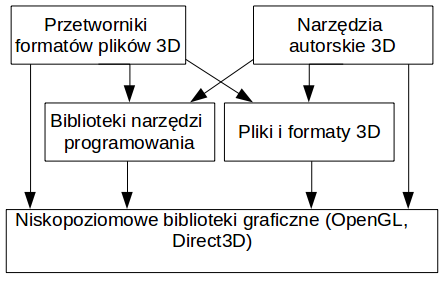
\includegraphics[width=7.0cm]{relacje.png}
 		\captionsetup{font={up, footnotesize}}
    	\caption{Relacje w narzędziach 3D.}
 		\label{rys5}
\end{figure}
Poniżej są przedstawione krótkie opisy najczęściej używanych formatów plików 3D. %przez kogo?%

\subsubsection{Collada}
Collada to format pliku 3D z rozszerzeniem .DAE, powszechnie jest używany do modelowania w grach komputerowych i filmografii. W całości opiera się na strukturalizowaną reprezentację w XML. Przechowuje wszystkie dane dotyczące modelu 3D, jeden z niewielu formatów wspierających kinematykę i informacje o cieniowaniu.\\
Struktura formatu zaczyna się w korzeniu zwanym COLLADA, który zawiera elementy mianowane bibliotekami i sceną. Element scena mieści w sobie odnośnik do rzeczywistego początku hierarchii sceny. Natomiast każdy element "biblioteka"\ składa się ze specjalnych zestawów danych dokładnie opisujących model: informacje o siatce (library\_geometries), obrazie (library\_images) itd. Taki podział jest bardzo wygodny pod względem odwoływania się do konkretnych sekcji.  
 %coś o parsowaniu XML?%

\subsubsection{STL}
STL (STereoLithography) jest jednym z najważniejszych formatów plików w dziedzinie druku 3D, tworzenia prototypów oraz komputerowo wspieranej produkcji. Rozszerzenie odpowiadające temu formatowi to .STL. Są dostępne oba rodzaje reprezentacji: tekstowy i binarny, przy czym binarny jest bardziej wykorzystywany ze względu na porównywalnie mały rozmiar plików. \\
W STL są pominięte takie dane jak wygląd, scena czy animacje. Jedyne ważne informacje w tym formacie to geometria obiektów, która jest zapisywana w postaci przybliżonej siatki trójkątów. Dla każdego trójkąta są przechowywane 2 rodzaje danych:
\begin{itemize}
\itemi współrzędne wierzchołków;
\itemi współrzędne normalnej, przy tym wektor powinien wskazywać na zewnątrz w odniesieniu do modelu 3D.
\end{itemize}
\begin{figure}[H]
		\centering
 		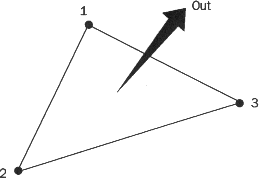
\includegraphics[width=5.0cm]{vertices-and-normal.png}
 		\captionsetup{font={up, footnotesize}}
    	\caption{Wierzchołki i normalna.}
 		\label{rys6}
\end{figure}
 Dotychczas jest to najprostszy i najbardziej ścisły format przechowywania informacji o modelu 3D. Wadą STL możnaby nazwać brak przechowywania danych o kolorach, ze względu na dynamiczny rozwój technologii druku pełnokolorowego \cite{stlinfo}.

\subsubsection{OBJ}
OBJ jest jednym z najbardziej znanych i wykorzystywanych formatów plików 3D, obecnie nabiera szczególnej wagi w druku 3D. Ten format przechowuje informacje o modelu w postaci tekstu ASCII (rozszerzenie .OBJ) bądź pliku binarnego (rozszerzenie .MOD) \cite{objinfo}.
Format binarny jest zastrzeżony i nieudokumentowany, dlatego poniżej zostanie opisana tylko postać tekstowa formatu. \\
OBJ wspiera dane o prostych, wielokątach, krzywych oraz powierzniach o różnych kształtach. Proste i wielokąty są opisywane poprzez wierzchołki, z których się składają. W przypadku krzywych oraz płaszczyzn kluczowymi są punkty kontrolne i inne niezbędne do opisu informacje, w zależności od typu krzywej. Ten format pliku 3D przybliża bądź oblicza doskładną siatkę bez drastycznego zwiększania rozmiaru pliku. Staje się to możliwe dzięki wykorzystaniu krzywych Beziera oraz metody NURBS (ang. Non-Uniform Rational Bezier Spline). \\
Format OBJ umożliwia również przechowywanie informacji o kolorach oraz teksturach modelu w towarzyszącym formacie MTL (ang. Material Template Library). Plik .OBJ, po sparowaniu z odpowiednim plikiem .MTL, tworzy realistyczny wielokolorowy teksturowany model. Plik MTL jest zapisywany w postaci tekstu ASCII definiującego właściwości materiałów, odbijania światła itd. Dodatkowo MTL wspiera mapy tekstur, w tym przypadku każdy wierzchołek siatki modelu 3D jest przyporządkowywany do dwuwymiarowego obrazu. 
%obrazek?: https://all3dp.com/obj-file-format-explained-cad-3d-printing/


\subsubsection{3DS}
3DS - to binarny format pliku początkowo wykorzystywany tylko w programie Autodesk 3D Studio. Plik binarny jest oparty o hierarchiczną strukturę "klocków"\ (ang. chunks), w której każdy fragment danych jest umieszczony w bloku z odpowiednim identyfikatorem. Pozwala to analizatorowi składni pominąć fragmenty, które nie są rozpoznawalne, oraz zapewnia możliwość rozszerzenia formatu. %https://pl.wikipedia.org/wiki/3ds
\\
3DS przechowuje tylko podstawowe informacje o geomertii, wyglądzie (kolory, tekstury i materiały), scenie oraz animacji. Gromadząc dane o scenie zapisuje położenie kamer i świateł, z wyjątkiem informacji o kierunkowych źródłach światła. Do przybliżenia kształtu obiektu w formacie 3DS używa się siatki trójkątów, ale liczba wierzchołków i wielokątów nie może przekraczać 65536($2^{16}$). 3DS jest obsługiwany praktycznie przez wszystkie pakiety oprogramowania 3D. Z względu na to, że jednak ten format zbiera tylko podstawowe informacje o modelu 3D, może on być uzupełniony o format MAX (obecnie zastąpiony formatem PRJ), który zawiera dodatkowe informacje specyficzne dla Autodesk 3DS Max, aby umożliwić całkowite zapisanie i załadowanie sceny.

\subsubsection{X3D}
Początkowo X3D nazywał się VRML (rozszerzenie pliku .WRL), z ang. Virtual Reality Modeling Language. Format został opracowany na potrzeby WWW (ang. World Wide Web), z czasem został zastąpiony przez X3D. Jest oparty o składnię XML. X3D wykorzystuje siatkę wielokątów do zakodowania kształtu modelu, umożliwia przechowywanie wyglądu i danych, które wiążą się z tym parametrem. Na przeciągu ostatnich lat rozwoju tego formatu zostały dodane: kodowanie NURBS powierzchni geometrii a także możliwość gromadzenia danych o scenie i animacjach.

\subsubsection{Porównanie formatów plików}
Poniższa tabela przedstawia porównanie opisanych formatów plików 3D pod względem różnorodności przechowywanych danych. 
\begin{savenotes}
\begin{table}[H]
\caption{Macierz funkcjonalności najpopularniejszych formatów plików 3D}
\centering
\footnotesize
\label{tab1}
  \begin{tabular}{!{\color{sapphire}\vrule width 1pt}c!{\color{black}\vrule width 1pt}c!{\color{black}\vrule width 1pt}c!{\color{black}\vrule width 1pt}c!{\color{black}\vrule width 1pt}c!{\color{black}\vrule width 1pt}c!{\color{black}\vrule width 1pt}c!{\color{black}\vrule width 1pt}c!{\color{black}\vrule width 1pt}c!{\color{black}\vrule width 1pt}c!{\color{black}\vrule width 1pt}c!{\color{sapphire}\vrule width 1pt}}
	\arrayrulecolor{sapphire}\hline
    \multirow{2}{*}{\bfseries Format} &
      \multicolumn{3}{c!{\color{black}\vrule width 1pt}}{\bfseries Geometria} &
      \multicolumn{3}{c!{\color{black}\vrule width 1pt}}{\bfseries Wygląd} &
      \multicolumn{3}{c!{\color{black}\vrule width 1pt}}{\bfseries Scena} &
     \multirow{2}{*}{\bfseries Animacje}\\
     \cline{2-10}
    & Przybl.\footnote{Przybliżona siatka}&Dokł.\footnote{Dokładna siatka}&CSG\footnote{CSG (ang. constructive solid geometry) – technika definiowania nowych brył poprzez łączenie innych brył}& Kolor& Materiał&Tekstura&Kamera&Światło&Pozycje& \\
    \hline
    Collada & X & X &  & X & X & X & X & X & X & X\\   
    \arrayrulecolor{black}
	\hline
    STL & X &  &  &  &  &  &  &  &  & \\
    \hline
    OBJ & X & X &  & X & X & X &  &  &  & \\
    \hline
    3DS & X &  &  & X & X & X & X & X & X & \\ 
    \hline
    X3D & X & X & X & X & X & X & X & X & X & X\\     
   \arrayrulecolor{sapphire}\hline
  \end{tabular}
\end{table}
\end{savenotes}
Z tabeli wynika, że najwięcej informacji przechowują formaty Collada i X3D. W niszej pracy dyplomowej zostanie wykorzystany format Collada, ze względu na strukturę oraz możliwość łatwego użycia w programie Blender.

\newpage
\subsection{Biblioteka OpenGL}
OpenGL (z ang. Open Graphics Library) jest potężnym systemem graficznym stanowiącym niejako pomost między programistą a sprzętem komputera. Procedury OpenGL umożliwiają rendorowanie obiektów o rożnych poziomach skomplikowania zaczynając od prostego punktu geometrycznego, linii lub wypełnionego wielokąta do utworzenia najbardziej złożonej, zakrzywionej powierzchni, oświetlonej i odwzorowanej teksturą. OpenGL pozwala programistom na dostęp do prymitywów geometrycznych i obrazowych, przekształcania modelu, oświetlenia i teksturowania, antyaliasingu i wielu innych funkcji. \\
OpenGL obsługuje aplikacje wizualizacji z obrazami 2D traktowanymi jako typy prymitywów, którymi można manipulować podobnie jak obiektami geometrycznymi 3D. Mimo że specyfikacja biblioteki definiuje konkretny potok przetwarzania graficznego, dostawcy platformy mają swobodę dostosowywania konkretnej implementacji OpenGL w celu osiągnięcia sprecyzowanych celów w zakresie kosztów i wydajności. Pojedyncze wywołania mogą być wykonywane na dedykowanym sprzęcie, uruchamiane jako procedury programowe w standardowym systemie CPU lub implementowane jako kombinacja zarówno specjalnych procedur sprzętowych, jak i programowych. Taka elastyczność implementacji skutkuje przyśpieszeniem renderowania, w dodatku jest powszechnie dostępna na wszystkich jednostkach od komputerów o niskich kosztach, po wysokiej klasy stacjach roboczych i superkomputerach \cite{openglofficial}.
\subsubsection{Potok przetwarzania}
\begin{figure}[H]
		\centering
 		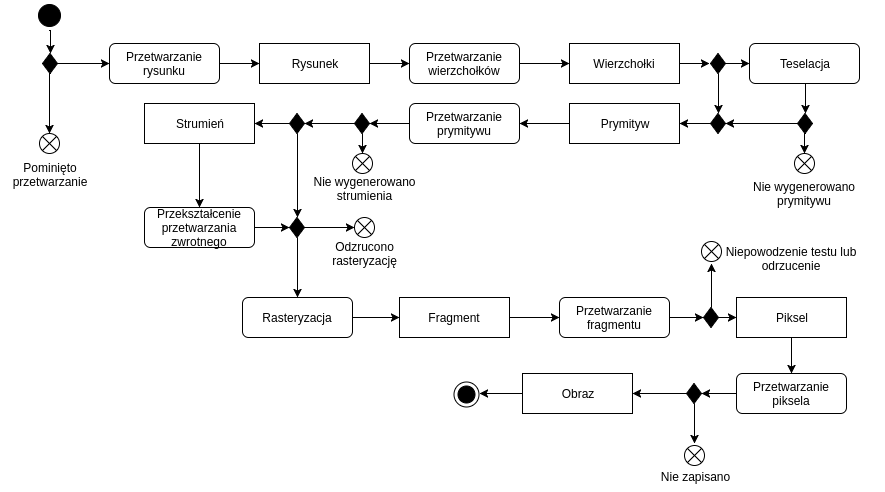
\includegraphics[width=15.5cm]{OpenGL.png}
 		\captionsetup{font={up, footnotesize}}
    	\caption{Schemat potoku przetwarzania.}
 		\label{rys7}
\end{figure}
W OpenGL wszystko jest przedstawione w przestrzeni trójwymiarowej, ale na ekranie obraz widzimy jako listę pikseli 2D, w związku z tym duża część pracy OpenGL polega na zmianie współrzędnych 3D na piksele 2D, które by pasowały do ekranu. Cały proces transformacji jest zarządzany poprzez potok graficzny OpenGL. Taki ciąg jest podzielony na poszczególne kroki, gdzie na wejściu są wymagane dane wyjściowe poprzedniego kroku. Każda z operacji jest dobrze sprecyzowana, gdyż mają one konkretną funkcję, i mogą być wykonane równolegle. Większość współczesnych kart graficznych posiada setki, czasmi tysiące, małych jąder procesowych do szybkiego przetwarzania danych wejściowych.

\subsubsection{Shadery}
Grupując poszczególne kroki w potoku przetwarzania OpenGL, otrzymuje się uproszczony schemat przetwarzania. Jest on przedstawiony na rys. \ref{rys8}.
\begin{figure}[H]
		\centering
 		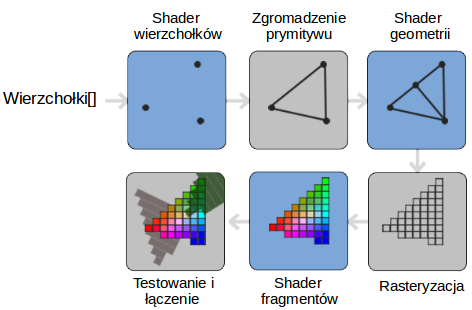
\includegraphics[width=11cm]{pipeline.png}
 		\captionsetup{font={up, footnotesize}}
    	\caption{Skrócony schemat potoku przetwarzania.}
 		\label{rys8}
\end{figure}
 
 Dla każdego kroku przetwarzania w celu przyśpieszenia obliczeń są uruchamiane nieduże programy w procesorze graficznym. Wspomniane nieduże programy są nazywane shaderami.\\
Shadery są pisane w języku w dużym stopniu podobnym do C - GLSL (ang. OpenGL Shading Language, język cieniowania OpenGL). GLSL jest dostosowany do wykorzystania w grafice, ponieważ zawiera przydatne funkcje skierowane na manipulacje wektorami i macierzami. Shadery zawsze zaczynają się od deklaracji wersji, następnie deklarowane są listy zmiennych wejściowych i wyjściowych, uniformy oraz ich główne funkcje. \\

\begin{itemize} 
\itemi Shader wierzchołków (ang. vertex shader). Pierwszym etapem ciągu graficznego jest przetwarzanie wierzchłków. Na wejściu jest przyjmowany jeden wierzchołek. Shader ma za zadanie transformację współrzędnych 3D do innych współrzędnych 3D. Taki program również pozwala robić podstawowe przetwarzanie atrybutów wierzchołka.
\itemi Zgromadzenie prymitywu (ang. primitive assembly). Jest to krok, który za dane wejściowe przyjmuje wszystkie wierzchołki (lub jeden, jeśli wybrana jest flaga GL\_POINTS ) z shadera wierzchołków. Na tym etapie przetwarzania kształtowane są prymitywy, wszystkie wierzchołki są grupowane do zadanego kształtu.
\itemi Shader geometrii (ang. geometry shader). Dane wyjściowe z poprzedniego kroku są przekazywane do shadera geometrii. Taki program przyjmuje jako argumenty wejściowe kolekcję wierzchołków, które tworzą zadany kształt oraz mogą generować inne, emitując nowe wierzchołki, tworząc nowe (lub inne) prymitywy. 
\itemi Rasteryzacja (ang. rasterization). Dane wyjściowe z shadera geometrii są podawane na wejście etapu rasteryzacji. W tym kroku uzyskane wcześniej prymitywy mapuje się na odpowiadające im piksele na ekranie ostatecznym. W wyniku, powstają fragmenty do przetwarzania w kolejnym kroku, ale zanim zostanie uruchomiony shader fragmentów, jest wykonywane przycinanie. Przyciannie pozwala odrzucić wszystkie fragmenty, które są poza zasięgiem obserwatora. Ów krok pozwala znacznie zwiększyć wydajność całego ciągu. Fragment w OpenGL zawiera wszystkie niezbędne dane do wyświetlenia pojedyńczego piksela.
\itemi Shader fragmentów. Głównym celem tego programu jest obliczenie końcowego koloru piksela i jest to zazwyczaj etap, na którym występują wszystkie zaawansowane efekty OpenGL. Z reguły shader fragmentów posiada wszystkie dane o scenie 3D (takie jak światła, cienie, kolor światła itp.), które są niezbędne dla określenia ostatecznej wartości koloru piksela.
\end{itemize}

\newpage
\subsection{Biblioteki do czytania i pisania modeli 3D}
Niestety, graficzne biblioteki niskiego poziomu takie jak OpenGL czy DirectX nie zapewnią żadnego mechanizmu do ładowania, zapisywania lub manipulowania modelami 3D. Dlatego, powstała potrzeba stworzenia nowych bibliotek ułatwiających te czynności. 
\subsubsection{Assimp}
Assimp (ang. Open Asset Import Library) to przenośna biblioteka do importowania różnych dobrze znanych formatów modeli 3D w jednolity sposób. Najnowsza wersja potrafi nie tylko czytać, ale również i zapisywać pliki 3D i dlatego nadaje się jako transformator modeli 3D do ogólnego zastosowania. Assimp jest napisana w języku C ++, istnieje również API (ang. Application Programming Interface) w języku C, a także jest powiązana z innymi językami programowania, w tym C \#, .net, Python i D.\\
Assimp ładuje wszystkie formaty modeli wejściowych do jednej prostej struktury danych w celu dalszego przetwarzania. Podstawowy zestaw funkcji jest rozszerzany przez różne narzędzia do przetwarzania końcowego. Przykładem rozszerzenia mogą posłużyć często potrzebne operacje, takie jak obliczanie wektorów normalnych i stycznych \cite{assimp}.
\subsubsection{lib3ds}
Lib3ds to darmowa alternatywa dla pakietu 3DS File Toolkit firmy Autodesk do zarządzania plikami 3DS. Ta biblioteka jest w całości napisana w języku C, wspierana przez takie platformy jak GNU, UNIX, Mac OS X, Microsoft Visual C++ 8.0. Jest łatwo integrowalna z biblioteką OpenGL \cite{lib3dsofficial}. \\
Celem lib3ds jest uproszczenie tworzenia filtrów do czytania i pisania plików formatu 3DS. Ta biblioteka jest obsługiwana na różnych rodzajach procesorów (big oraz little endian), wspiera moduły wektorowe, kwaterniony, macierze, proste struktury danych, które można łatwo modyfikować, ocenę wszystkich danych animacji. Istnieje możliwość załadowania większości fragmentów 3DS, sekcje: materiały, kamera, światło, siatka i klucze \cite{lib3dsdirectory}.

\newpage
\subsection{ALICE}
ALICE ( ang. A Large Ion Collider Experiment, czyli Wielki Eksperyment Zderzacza Jonów) jest jednym z największych na świecie eksperymentów fizycznych. Celem tego eksperymentu jest pomiar zderzeń ciężkich jonów przy najwyższych osiągalnych obecnie energiach przy użyciu detektora na Wielkim Zderzaczu Hadronów w międzynarodowym laboratorium fizyki cząstek CERN w Genewie. \\
Detektor ALICE został zaprojektowany tak, aby w jak najbardziej kompletny sposób badać cząstki powstałe w kolizjach, które mają miejsce w środku akceleratora. Do zrealizowania założeń, używa sie wielu warstw różnych detektorów, z których każda dostarcza innych informacji o przebiegu zderzenia. Dane są gromadzone w sposób umożliwiający zrekonstruowanie i zbadanie ewolucji systemu cząstek w przestrzeni i czasie \cite{aliceofficial}. 

\subsubsection{Eksperyment}
W ekstremalnych warunkach temperatury i (lub) gęstości materia hadronowa topi się w osoczu wolnych kwarków i gluonów - tak zwanej plazmy kwarkowo-gluonowej (ang. quark–gluon plasma - QGP). Aby stworzyć odpowiednie warunki w laboratorium, ciężkie jony (np. cząstki ołowiu) przyśpiesza się do niemal prędkości światła, po czym jest powodowana kolizja. Kluczowym rozważaniem dotyczącym eksperymentu ALICE jest zdolność do badania chromodynamiki kwantowej ( ang.  quantum chromodynamics - QCD) i kwarków w tych ekstremalnych warunkach. Odbywa się to przy użyciu cząstek, utworzonych wewnątrz gorącej objętości podczas jej rozszerzania się i ochładzania. Cząstki te żyją wystarczająco długo, aby dotrzeć do wrażliwych warstw detektora zlokalizowanych wokół obszaru oddziaływania. Fizyka w ALICE polega na tym, żeby być w stanie zidentyfikować wszystkie z nich (tj. określić, czy są to elektrony, fotony, piony itd.), czy też określić ich ładunek. Wiąże się to w większości z różnymi sposobami oddziaływania cząstek z materią \cite{aliceexperiment}.

\subsubsection{Ślady cząstek i detektory}
Zespół detektorów cylindrycznych (od wewnątrz na zewnątrz: ITS\footnote{The Inner Tracking System}  Drift, ITS Strips, TPC\footnote{The ALICE Time Projection Chamber}, TRD\footnote{The ALICE Transition Radiation Detector}) mierzy w wielu punktach (ponad 100 tylko dla TPC) przejście każdej cząstki przenoszącej ładunek elektryczny tak, że trajektoria jest dokładnie znana. Detektory ALICE są osadzone w polu magnetycznym (wytwarzanym przez duży czerwony magnes), wyginając w ten sposób trajektorie cząstek: z krzywizny śladów można znaleźć ich pęd. ITS jest tak precyzyjny, że cząstki, które są generowane przez rozkład innych cząstek o bardzo krótkim czasie życia można zidentyfikować, widząc, że nie pochodzą one z punktu, w którym nastąpiła interakcja ("wierzchołek"\ zdarzenia) \cite{trackingparticles}.

\begin{figure}[H]
		\centering
 		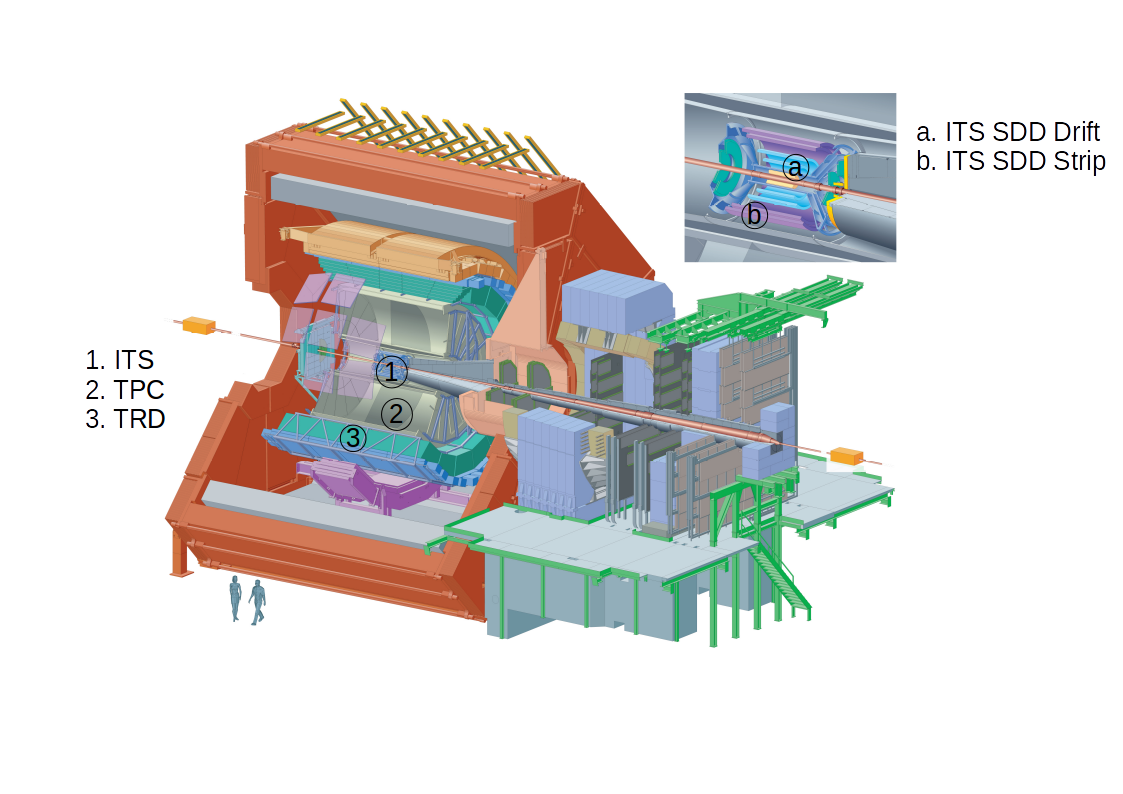
\includegraphics[width=15.5cm]{detector.png}
 		\captionsetup{font={up, footnotesize}}
    	\caption{Detektor ALICE.}
 		\label{rys9}
\end{figure}
\newpage
\section{Projekt}
\subsection{Wymagania}
\subsubsection{funkcjonalne}
\subsubsection{niefunkcjonalne}

\subsection{Diagramy}
\subsubsection{przypadków użycia}
\subsubsection{klas}

\newpage
\subsection{Technologie}
\subsubsection{GLFW} 
GLFW jest to Open Source, multipatformowa biblioteka dla OpenGL, OpenGL ES. Zapewnia ona proste API do tworzenia okien, kontekstów i powierzchni, odbierania danych wejściowych i zdarzeń. GLFW jest napisana w C posiada macierzystą obsługę systemów Windows, macOS i wielu systemów uniksopodobnych, takich jak Linux i FreeBSD. 
Zalety GLFW :
\begin{enumerate}
\item Tworzy okno i cały kontekst OpenGL używając wywołania tylko 2 funkcji.
\item Obsługuje OpenGL, OpenGL ES, Vulkan i powiązane opcje, flagi oraz rozszerznia.
\item Obsługuje wiele okien, wiele monitorów, ramp o wysokiej rozdzielczości DPI i gamma.
\item Obsługuje klawiatuę, mysz, gamepad, czas i okna zdarzenia, poprzez odpytywanie lub callback.
\item Dostęp do rodzimych obiektów i opcji kompilacji dla specyficznych funkcji platformy.
\end{enumerate} 

\subsubsection{GLEW}
The OpenGL Extension Wrangler Library (GLEW) jest wieloplatformową biblioteką C / C ++. GLEW zapewnia efektywne mechanizmy wykonawcze do określania, które rozszerzenia OpenGL są obsługiwane na docelowej platformie. Funkcje jądra i rozszerzenia OpenGL są widoczne w pojedynczym pliku nagłówkowym. GLEW została przetestowany na różnych systemach operacyjnych, w tym na systemach Windows, Linux, Mac OS X, FreeBSD i Solaris.
Podczas tworzenia wizualizacji została użyta wersja statyczna GLEW, czyli glew32s.lib. \footnote{http://glew.sourceforge.net/}

\subsubsection{GLM}
OpenGL Mathematics (GLM) jest nagłówkiem tylko do biblioteki matematycznej C++ dla oprogramowania graficznego opartego na specyfikacjach języka GLSL, udostępnia klasy i funkcje zaprojektowane i zaimplementowane z użyciem tych samych konwencji nazewnictwa jak w GLSL. Mimo to GLM nie jest ograniczony tylko do cech GLSL. System rozszerzenia, oparty na konwencjach rozszerzeń GLSL, zapewnia dodatkowe możliwości: przekształcenia macierzy i kwaternionów, pakowanie danych, liczby losowe itp. \\
Ta biblioteka działa doskonale z OpenGL, ale zapewnia również współdziałanie z innymi bibliotekami i SDK innych firm. Jest dobrym kandydatem do oprogramowania renderowania (raytracing czy rasteryzacji), przetwarzania obrazu, symulacji fizycznych i dowolnego kontekstu programowania, który wymaga prostej i wygodnej biblioteki matematycznej. 
\footnote{http://glm.g-truc.net/0.9.8/index.html}




\newpage
\section[Część weryfikacyjna]{Część weryfikacyjna/Wyniki eksperymentów/Wyniki symulacji}

\section[Zakończenie]{Zakończenie/Wnioski/Podsumowanie}


\newpage
\section[Przykłady]{Przykłady rysunków, tabel itp.}
\subsection{Listowanie}
Listuje się w sposób następujący:
\begin{itemize}
	\itemi pierwszy poziom listy - element pierwszy,
	\itemi pierwszy poziom listy - element drugi,
	\begin{itemize}
		\itemii drugi poziom listy - element pierwszy,
		\itemii drugi poziom listy - element drugi,
		\itemii drugi poziom listy - element trzeci,
		\begin{itemize}
			\itemiii trzeci (ostatni) poziom listy - element pierwszy,
			\itemiii trzeci (ostatni) poziom listy - element drugi,
			\itemiii trzeci (ostatni) poziom listy - element trzeci,
		\end{itemize}
		\itemii drugi poziom listy - element czwarty,
		\end{itemize}
	\itemi pierwszy poziom listy - element trzeci,
	\itemi pierwszy poziom listy - element czwarty.
\end{itemize}

\begin{table}[H]
\caption{Kod źródłowy programu. Aproksymacja krzywych Beziera.}
\label{tab2}
\begin{lstlisting}[frame=single]
GLfloat bezier(float t, GLfloat P0,
                  GLfloat P1, GLfloat P2, GLfloat P3) {
  // Cubic bezier Curve
  GLfloat point = (pow((1-t), 3.0) * P0) +
    (3 * pow((1-t),2) * t * P1) +
    (3 * (1-t) * t * t * P2) +
    (pow(t, 3) * P3);
  return point;
}

void drawStuff() {
  midpoint_x = bezier(P0.x, P1.x, P2.x, P3.x, t);
  midpoint_y = bezier(P0.y, P1.y, P2.y, P3.y, t);

  drawPoint(midpoint_x, midpoint_y);
}
\end{lstlisting}
\end{table}

\newpage
\bibliographystyle{plain} % bibliography style
\bibliography{bibliography} % add bibliography


\end{document}
